\documentclass[11pt,a4paper,oneside]{report}             % Single-side
%\documentclass[11pt,a4paper,twoside,openright]{report}  % Duplex

%\PassOptionsToPackage{chapternumber=Huordinal}{magyar.ldf}
\usepackage{t1enc}
\usepackage[utf8]{inputenc}
%\usepackage{newunicodechar} 
%\DeclareUnicodeCharacter{FFFD}{?????}
\usepackage{graphicx}
\usepackage{float}
\usepackage{amsmath}
\usepackage{amssymb}
\usepackage{enumerate}
\usepackage[thmmarks,amsmath]{ntheorem}
\usepackage{graphics}
\usepackage{epsfig}
\usepackage{listingsutf8}
\usepackage{color}
\usepackage{lastpage}
\usepackage{anysize}
\usepackage[hungarian]{babel}
\usepackage{sectsty}
\usepackage{setspace}  % Ettol a tablazatok, abrak, labjegyzetek maradnak 1-es sorkozzel!
\usepackage[hang]{caption}
\usepackage{hyperref}
\usepackage{caption}
\usepackage{subfig}
%--------------------------------------------------------------------------------------
% Main variables
%--------------------------------------------------------------------------------------
\newcommand{\vikszerzo}{boa}
\newcommand{\vikkonzulens}{Konzulens}
\newcommand{\vikcim}{Információkereső rendszer fejlesztése rövid hírekhez}
\newcommand{\viktanszek}{Méréstechnika és Információs Rendszerek Tanszék}
\newcommand{\vikdoktipus}{Szakdolgozat}
\newcommand{\vikdepartmentr}{BME/MIT}

%--------------------------------------------------------------------------------------
% Page layout setup
%--------------------------------------------------------------------------------------
% we need to redefine the pagestyle plain
% another possibility is to use the body of this command without \fancypagestyle
% and use \pagestyle{fancy} but in that case the special pages
% (like the ToC, the References, and the Chapter pages)remain in plane style

\pagestyle{plain}
%\setlength{\parindent}{0pt} % áttekinthetőbb, angol nyelvű dokumentumokban jellemző
%\setlength{\parskip}{8pt plus 3pt minus 3pt} % áttekinthetőbb, angol nyelvű dokumentumokban jellemző
\setlength{\parindent}{12pt} % magyar nyelvű dokumentumokban jellemző
\setlength{\parskip}{0pt}    % magyar nyelvű dokumentumokban jellemző

\marginsize{35mm}{25mm}{15mm}{15mm} % anysize package
\setcounter{secnumdepth}{0}
\sectionfont{\large\upshape\bfseries}
\setcounter{secnumdepth}{4}
\singlespacing
\frenchspacing

%--------------------------------------------------------------------------------------
%	Setup hyperref package
%--------------------------------------------------------------------------------------
\hypersetup{
    bookmarks=true,            % show bookmarks bar?
    unicode=false,             % non-Latin characters in Acrobat’s bookmarks
    pdftitle={\vikcim},        % title
    pdfauthor={\vikszerzo},    % author
    pdfsubject={\vikdoktipus}, % subject of the document
    pdfcreator={\vikszerzo},   % creator of the document
    pdfproducer={Producer},    % producer of the document
    pdfkeywords={keywords},    % list of keywords
    pdfnewwindow=true,         % links in new window
    colorlinks=true,           % false: boxed links; true: colored links
    linkcolor=black,           % color of internal links
    citecolor=black,           % color of links to bibliography
    filecolor=black,           % color of file links
    urlcolor=black             % color of external links
}

%--------------------------------------------------------------------------------------
% Set up listings
%--------------------------------------------------------------------------------------
\lstset{
	basicstyle=\scriptsize\ttfamily, % print whole listing small
	keywordstyle=\color{black}\bfseries\underbar, % underlined bold black keywords
	identifierstyle=, 					% nothing happens
	commentstyle=\color{white}, % white comments
	stringstyle=\scriptsize\sffamily, 			% typewriter type for strings
	showstringspaces=false,     % no special string spaces
	aboveskip=3pt,
	belowskip=3pt,
	columns=fixed,
	backgroundcolor=\color{lightgray},
	literate={ö}{{\"{o}}}1 {Ö}{{\"{O}}}1 {ü}{{\"{u}}}1 {Ü}{{\"{u}}}1 {ó}{{\'{o}}}1 {Ó}{{\'{O}}}1 {ő}{{\H{o}}}1 {Ő}{{\H{O}}}1 {ú}{{\'{u}}}1 {Ú}{{\'{U}}}1 {é}{{\'{e}}}1 {É}{{\'{E}}}1 {á}{{\'{a}}}1 {Á}{{\'{A}}}1 {ű}{{\H{u}}}1 {Ű}{{\H{U}}}1 {í}{{\'{i}}}1 {Í}{{\'{I}}}1
} 		
\def\lstlistingname{lista}	

%--------------------------------------------------------------------------------------
%	Some new commands and declarations
%--------------------------------------------------------------------------------------
\newcommand{\code}[1]{{\upshape\ttfamily\scriptsize\indent #1}}

% define references
\newcommand{\figref}[1]{\ref{fig:#1}.}
\renewcommand{\eqref}[1]{(\ref{eq:#1})}
\newcommand{\listref}[1]{\ref{listing:#1}.}
\newcommand{\sectref}[1]{\ref{sect:#1}}
\newcommand{\tabref}[1]{\ref{tab:#1}.}

\DeclareMathOperator*{\argmax}{arg\,max}
%\DeclareMathOperator*[1]{\floor}{arg\,max}
\DeclareMathOperator{\sign}{sgn}
\DeclareMathOperator{\rot}{rot}
\definecolor{lightgray}{rgb}{0.95,0.95,0.95}

\author{\vikszerzo}
\title{\viktitle}
\includeonly{
	project,%
	titlepage,%
	declaration,%
	abstract,%
	introduction,%
	chapter1,%
	chapter2,%
	chapter3,%
	chapter4,%
	acknowledgement,%
	appendices,%
}
%--------------------------------------------------------------------------------------
%	Setup captions
%--------------------------------------------------------------------------------------
\captionsetup[figure]{
%labelsep=none,
%font={footnotesize,it},
%justification=justified,
width=.75\textwidth,
aboveskip=10pt}

\renewcommand{\captionlabelfont}{\small\bf}
\renewcommand{\captionfont}{\footnotesize\it}

%--------------------------------------------------------------------------------------
% Table of contents and the main text
%--------------------------------------------------------------------------------------
\begin{document}
\singlespacing
\include{guideline}
%--------------------------------------------------------------------------------------
% Feladatkiiras (a tanszeken atveheto, kinyomtatott valtozat)
%--------------------------------------------------------------------------------------
\clearpage
\begin{center}
\large
\textbf{FELADATKIÍRÁS}\\
\end{center}

A természetes nyelvű szövegek feldolgozása az informatika egy régi és egyre nagyobb fontossággal bíró területe. Az információkeresés és -kinyerés, az üzleti intelligencia rendszerek, a természetes nyelvű ember-gép interfészek, a közösségi média álhíreinek detektálása, vagy például történeti és irodalmi szövegek számítógépes analízise mind olyan területek, ahol ezeknek a módszereknek egyre nagyobb szerep jut.

A feladat egy olyan rendszer megvalósítása, amely az internetről származó rövid, természetes nyelvű szöveges hírekből felépített korpuszon képes információkeresési és -kinyerési feladatok megoldására. A rendszernek alkalmasnak kell lennie egy szövegbázis betöltésére (közben a releváns tartalmak kiválasztására), majd az így létrehozott korpuszon különféle elemzési és keresési feladatok megoldására, pl. entitásfelismerés, szemantikus annotálás, relevancialapú dokumentum-részletek keresése, információkinyerés, kérdés-megválaszolás stb. A feladat megoldása során azt is meg kell vizsgálni, hogy az elmúlt években megjelent nagy nyelvi modellek (large language models) alkalmazásának milyen lehetőségei vannak ezen a területen.

A hallgató munkájának a következőkre kell kiterjednie:
\begin{itemize}
	\item a feladatkiíráshoz hasonló célú megoldások felkutatása és megismerése,
	\item a rendszer fejlesztésére és tesztelésére alkalmas dokumentumgyűjtemény létrehozása,
	\item a fentebb megfogalmazott feladatokat megoldó alkalmazás tervezése és megvalósítása,
	\item a nagy nyelvi modellek lehetséges alkalmazásainak vizsgálata,
	\item teljesítménymértékek meghatározása az alkalmazás működésének kiértékelésére,
	\item információkeresési kísérletek futtatása, az alkalmazás működésének értékelése.
\end{itemize}





\pagenumbering{arabic}
\onehalfspacing
%--------------------------------------------------------------------------------------
%	The title page
%--------------------------------------------------------------------------------------
\begin{titlepage}
\begin{center}

\includegraphics[width=60mm,keepaspectratio]{figures/BMElogo.png}\\
\vspace{0.3cm}
\textbf{Budapesti Műszaki és Gazdaságtudományi Egyetem}\\
\textmd{Villamosmérnöki és Informatikai Kar}\\
\textmd{\viktanszek}\\[5cm]

\vspace{0.4cm}
{\huge \bfseries \vikcim}\\[0.8cm]
\vspace{0.5cm}
\textsc{\Large \vikdoktipus}\\[4cm]

\begin{tabular}{cc}
 \makebox[7cm]{\emph{Készítette}} & \makebox[7cm]{\emph{Konzulens}} \\
 \makebox[7cm]{\vikszerzo} & \makebox[7cm]{\vikkonzulens}
\end{tabular}

\vfill
{\large \today}
\end{center}
\end{titlepage}



\tableofcontents\vfill
%--------------------------------------------------------------------------------------
% Nyilatkozat
%--------------------------------------------------------------------------------------
\begin{center}
\large
\textbf{HALLGATÓI NYILATKOZAT}\\
\end{center}

Alulírott \emph{\vikszerzo}, szigorló hallgató kijelentem, hogy ezt a szakdolgozatot meg nem engedett segítség nélkül, saját magam készítettem, csak a megadott forrásokat (szakirodalom, eszközök stb.) használtam fel. Minden olyan részt, melyet szó szerint, vagy azonos értelemben, de átfogalmazva más forrásból átvettem, egyértelműen, a forrás megadásával megjelöltem.

Hozzájárulok, hogy a jelen munkám alapadatait (szerző(k), cím, angol és magyar nyelvű tartalmi kivonat, készítés éve, konzulens(ek) neve) a BME VIK nyilvánosan hozzáférhető elektronikus formában, a munka teljes szövegét pedig az egyetem belső hálózatán keresztül (vagy autentikált felhasználók számára) közzétegye. Kijelentem, hogy a benyújtott munka és annak elektronikus verziója megegyezik. Dékáni engedéllyel titkosított diplomatervek esetén a dolgozat szövege csak 3 év eltelte után válik hozzáférhetővé.

\begin{flushleft}
\vspace*{1cm}
Budapest, \today
\end{flushleft}

\begin{flushright}
 \vspace*{1cm}
 \makebox[7cm]{\rule{6cm}{.4pt}}\\
 \makebox[7cm]{\emph{\vikszerzo}}\\
 \makebox[7cm]{hallgató}
\end{flushright}
\thispagestyle{empty}

\vfill
\clearpage
\thispagestyle{empty} % an empty page


%----------------------------------------------------------------------------
% Abstract in hungarian
%----------------------------------------------------------------------------
\chapter*{Kivonat}\addcontentsline{toc}{chapter}{Kivonat}

Ebben a szakdolgozatban egy információ kinyerő rendszer fejlesztését járom körbe magyar nyelvű újságcikkeken... 

\vfill

%----------------------------------------------------------------------------
% Abstract in english
%----------------------------------------------------------------------------
\chapter*{Abstract}\addcontentsline{toc}{chapter}{Abstract}

In this thesis I present the development of an information retrieval system for news articles written in the Hungarian language.

\vfill


\chapter{Bevezető}

\section{Feladat háttere}

Egyre több szöveges tartalom születik az interneten, ezért aki arra vállalkozik, hogy ezekből manuálisan információt nyerjen ki, egyre nehezebb problémával találja szembe magát. Az én feladatom egy olyan rendszer fejlesztése, amely automatizált módon képes számos információ-kinyeréssel kapcsolatos feladat ellátására.

\section{Célok}

Célom egy olyan információkinyerő rendszer fejlesztése volt, ami képes számos monoton feladat ellátására, mint például a szövegklasszifikáció, kulcsszó- és entitásfelismerés, valamint a szöveg kontextusában rejlő entitások közti kapcsolatra utaló információ kinyerése. A rendszer lényeges részét képezi egy webes felület, amely lehetőséget biztosít a felhasználóknak a szoftver által végzett döntések ellenőrzésére és javítására.

A feladatot internetről származó hírek szövegén szerettem volna megoldani, ezért ilyen adatok gyűjtésére és tisztítására is szükség volt. Az összeállított korpusz segítségével akartam olyan modelleket tanítani, amik megoldanak emberek számára időigényes feladatokat, legalább olyan pontossággal, hogy az később segítséget jelentsen.

A rendszer fejlesztése során különös figyelmet fordítottam arra, hogy az legyen képes a legújabb nyelvtechnológiai megoldások - mint például a nagy nyelvi modellek - integrálására. Ez amellett, hogy lehetőséget biztosít eddig nehezen megoldható feladatok támogatására, új nehézségeket is felvet az erőforrásigény kapcsán.

A célkitűzések között szerepelt továbbá teljesítménymértékek meghatározása, hogy objektíven értékelhető legyen a rendszer pontossága. Ez magában foglalta különböző pontosságot mutató kísérletek végrehajtását és a rendszer egyes komponenseinek futási idejének mérését.

\section{Részfeladatok}

\subsection{Klasszifikáció}

%Mivel a feladat korrupcióval kapcsolatos cikkek szövegével kapcsolatos, első lépésként fontos megállapítani az egyes cikkekről, hogy ilyen témát dolgoznak-e fel, ebben segít a szövegklasszifikáció. Ez egy szövegelemzési eljárás, ami gépi tanulás segítségével képes egy adott szöveget osztályokba sorolni. Aszerint, hogy hány lehetséges osztály közül kell választani megkülönböztetünk bináris (két osztály) és multi-label (kettőnél több osztály) klasszifikációt. Jelen esetben a feladat csak azt követeli meg, hogy az adott szövegről eldöntsük beleillik-e egy konkrét témába, így elegendő a bináris klasszifikáció alkalmazása.

Mivel a feladat nem általános, hanem témaspecifikus újságcikkek szövegével kapcsolatos, első lépésként fontos megállapítani az egyes cikkekről, hogy olyan témát dolgoznak-e fel, ami a feladat szempontjából érdekes, ebben segít a szövegklasszifikáció. Ez egy szövegelemzési eljárás, ami gépi tanulás segítségével képes egy adott szöveget osztályokba sorolni. Aszerint, hogy hány lehetséges osztály közül kell választani megkülönböztetünk bináris (két osztály) és multi-label (kettőnél több osztály) klasszifikációt. Jelen esetben a feladat csak azt követeli meg, hogy az adott szövegről eldöntsük beleillik-e egy konkrét témába, így elegendő a bináris klasszifikáció alkalmazása.

A klasszifikáció kimenete azonban nem csak osztály lehet, sok módszer lehetőséget nyújt arra is, hogy az egyes osztályok modell által vélt valószínűségét is elárulja. Ez a kiegészítő információ felhasználható arra, hogy a klasszifikáció eredményét hangoljuk azzal, hogy pozitív eredmény esetén 50\%-nál nagyobb valószínűséget követelünk meg az elfogadáshoz, vagy épp fordítva.

% masik cikk hianyzik
\subsection{Névelemfelismerés és -klasszifikáció}

Az információkinyerés során egy kifejezetten fontos lépés a névelemfelismerés (Named Entity Recognition). Ez a szövegben előforduló entitások (például: személyek, intézmények, helyszínek) kinyerése és ellátása egy típusára utaló címkével.

Ez a folyamat csupán szövegrészleteket azonosít és adja meg az ott talált névelem típusát, így könnyen előfordulhat, hogy a felismert szövegrész nem egy teljes név, hanem annak csupán egy része: kereszt- vagy vezetéknév.

Az adatbázis bővítése szempontjából nem elegendő a névelemeket azonosítani, azokat még tovább kell szűrni a relevanci alapján, ami egy névelem klasszifikációs feladat. Emellett ebben a részfeladatban csökkentem a névelemek listáját a teljes nevekre.

\subsection{Kulcsszavak kinyerése}

A kulcsszókinyerés alatt általában a szövegben előforduló szavak frekvencia alapján való kiválasztását szokták érteni (például TF-IDF módszer). Azonban előfordulhat ennél tágabb definíciója a kulcsszónak, amikor nem feltétlenül szerepel az adott kulcsszó a szövegben és helyette egy előre meghatározott listából kell kiválasztani.

Ha a lehetséges kulcsszavak listája előre ismert ez a kulcsszókinyerés értelmezhető egy nagyon sok osztályos szöveg-klasszifikációs feladatként is.

\subsection{Névelemek közti kapcsolat kinyerése}

A korábbi lépésben megszerzett személyek és intézmények közötti összefüggések névelem-névelem-kapcsolat hármasokkénti kinyerése is cél. A névelem esetében fontos, hogy a teljes nevet tartalmazza, a kapcsolat viszont szabad szöveg. Ezen kapcsolatok kinyerése magában hordozza a tévedés lehetőségét, ezért segít, ha szövegkörnyezetet is csatolunk melléjük. Emellett manapság a generatív nagy nyelvi modellek már arra is lehetőséget adnak, hogy egy indoklást is rendeljünk a kinyert hármashoz.

\begin{figure}[H]
	\centering
	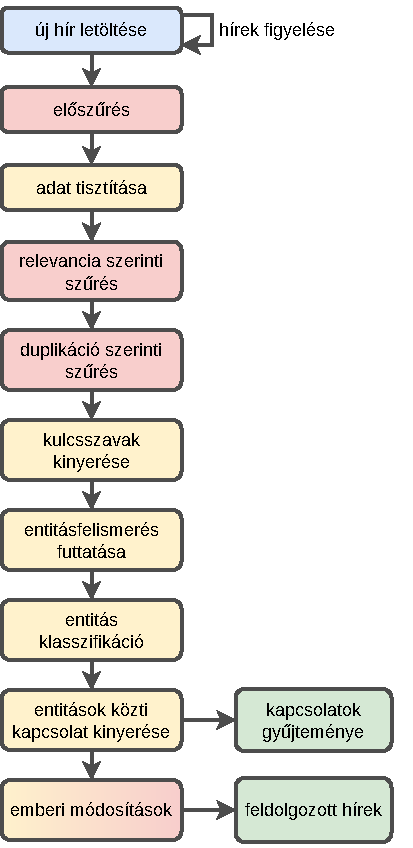
\includegraphics[width=100mm,keepaspectratio]{figures/flowchart.pdf}
	\caption{Rendszer működését bemutató folyamatábra}
\end{figure}

\chapter{Kapcsolódó megoldások}

\section{Technológiák bemutatása}
% bevezetes ilyen modszere altal transf

A modern szövegelemzési és nyelvfeldolgozási módszerek az elmúlt évtizedben jelentős fejlődésen mentek keresztül, ami elsősorban a transformer architektúrának és az előtanított nagy nyelvi modelleknek köszönhető \cite{transformer}. A szóvektorokra építő folyamatokat felváltotta az általános nagy nyelvi modellek feladatspecifikus finomhangolása.

\subsection{BERT}

2018-ban nagy áttörést jelentett a természetes nyelvű szövegelemzés területének a transformer architektúrát alkalmazó BERT modell megjelenése \cite{bert}. Ez encoder mechanizmust használ a szöveg reprezentálására, ami képes többek között klasszifikációs, névelem felismerés és kérdés-válaszolás feladatok megoldására is.

Nagy áttörést jelentett 2020-ban a magyar nyelvű szövegelemzés számára az első magyar nyelvű BERT modell, a huBERT \cite{Nemeskey:2021a} megjelenése. Ez egy BERT-Base típusú modell, ami 9 milliárd tokent tartalmazó magyar nyelvű szövegen lett tanítva. Számos magyar nyelvi benchmarkon jobban teljesít, mint a több-nyelvű BERT modellek.

\subsection{GPT}

A nagy nyelvi modellek következő generációját a szöveggenerálási feladatra tanított GPT modellek jelentették \cite{gpt1}. Ezek szintén a transformer architektúrát használják, viszont az encoder oldal mellett egy decoder-t is tartalmaznak. A BERT-el ellentétben ezt csak a következő token megtippelésre tanították, viszont szöveggeneráló képessége miatt képes sokféle feladatot elsajátítani finomhangoláson keresztül \cite{gpt2}.

A generatív nyelvi modellek közt nagy újításnak számított a GPT-3, melyről kiderült, hogy finomhangolás nélkül is képes feladatokat megoldani néhány példa (few-shot) alapján vagy akár példák nélkül (zero-shot) is \cite{gpt3}. Ennek a felfedezésnek a továbbviteleként született az InstructGPT, ami természetes nyelven megfogalmazott instrukciók/kérdések megválaszolására lett finomhangolva \cite{instructgpt}. A GPT-3 és az InstructGPT utódjaiként a GPT-4 és a ChatGPT sokat javítottak elődjeikhez képest, már szinte emberi szinteken teljesítve több feladatban is \cite{gpt4}.

\subsection{LoRA}

Ahogy nagy nyelvi modellek egyre elterjedtebbé váltak az utóbbi pár évben, megnőtt az igény ezeknek a finomhangolására, de egy klasszikus finomhangolás hosszú és erőforrásigényes procedúra. Ennek orvoslására találták ki a LoRA \cite{hu2022lora} finomhangolást, ami befagyasztja az előtanított nyelvi modell súlyait és annak kiválasztott részeit módosítja csak. A finomhangolás ezen kiválasztott súlyokat tartalmazó mátrixokat dekomponálja két kisebb mátrixszá, ezzel tovább csökkentve a hangolandó paramétereke számát. Ez a technika a hagyományos módszerhez képest akár harmadára is csökkentheti a szükséges memóriahasználatot és jóval kevesebb időt vesz igénybe.

\begin{figure}[H]
	\centering
	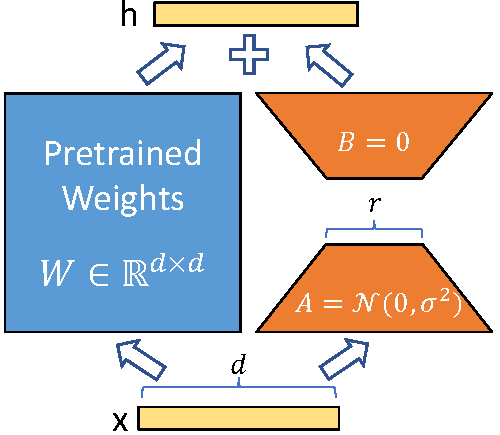
\includegraphics[width=0.49\textwidth]{figures/figure1.pdf}
	\caption{LoRA működése \cite{hu2022lora}}
\end{figure}

A LoRA használata a kisebb erőforrásigényen kívül azzal az előnnyel is jár, hogy a finomhangolás során keletkezett LoRA adapterek (súly módosítások) kevés helyet foglalnak a memóriában. Ha az alap modell már be van töltve a LoRA részek gyorsan cserélhetők futás közben, így megtehetjük, hogy feladatonként külön LoRA adaptert hangolunk és futás közben váltogatunk köztük.

Habár a technológia eredetileg nyelvi modellekhez lett kitalálva, képgeneráló modellekhez is adaptálták.

\subsection{QLoRA}

A LoRA módszerre épitve kutatók további fejlesztéseket dolgoztak ki LoRA adapterek hangolására alacsonyabb erőforrásigény elérése céljából a modell súlyainak kvantizálásával. A súlyok kvantizálása tömörítésként is felfogható és nagy (nyelvi) modelleknek arra a jól ismert tulajdonságára épít, hogy a súlyaik pazarló (nem optimális) módon tárolnak információt.

A QLoRA három fő innovatív módszer kombinációja:
\begin{enumerate}
	\item \textbf{4-bites NormalFloat}: kvantizációhoz használt adattípus, ami bizonyítottan optimális normál eloszlású súlyok esetén
	\item \textbf{Dupla Kvantizálás} (Double Quantization): egy módszer, ami a kvantizációs konstansokat kvantizálja, ezzel átlagosan 0.37 bitet spórol meg paraméterenként
	\item \textbf{Lapozott Optimalizálók} (Paged Optimizers): a neurális hálók optimalizáláshoz szükséges memória egy részét RAM-ban tárolja időlegesen, amivel a hosszabb szövegek miatti hirtelen memória-ingadozás esetén bekövetkező memória-túllépést ki lehet küszöbölni
\end{enumerate}

A QLoRA leglényegesebb újítása a LoRA-hoz képest tehát az, hogy az eredeti modell súlyait 4 bites számokkal tölti be 16 bit helyett, viszont közben az adaptert 16 biten hangolja.

\subsection{transformers (könyvtár)}

A transformers könyvtár \cite{transformers} egy egyszerű fejlesztői felületet ad, amin keresztül könnyen használhatók előtanított modellek háttérrendszertől (PyTorch, TensorFlow, JAX) függetlenül. A használat mellett a szoftvercsomag finomhangolást is támogat a legfrissebb fejlesztéseket (LoRA, QLoRA) beépítve. 

A könyvtár fejlesztői egy modellek és adathalmazok megosztását lehetővé tevő platformot is létrehoztak Hugging Face Hub néven. Ez a transformers-be integrálva egyszerűen hozzáférhetővé tett rengeteg különböző modellt fejlesztők számára.

\subsection{llama.cpp}

A transformer architektúra, amit a nagy nyelvi modellek többsége követ párhuzamosítható műveletek végzésére épül és emiatt leghatékonyabban videokártyákon (vagy speciális hardware-en) használható. Azonban GPU-k bérlése költséges és egyes alkalmazásoknál nem jelent problémát a késleltetés.

A llama.cpp egy generatív nyelvi modellek (elsősorban) processzoron való futtatására optimalizált szoftver. Alacsony szintű C/C++ nyleven lett fejlesztve és külön optimalizálták az egyes CPU architektúrákra, támogatva a SIMD operációkat.

\subsection{SpaCy}
Szövegek nyelvtani elemzésére számos módszert kidolgoztak, ezeknek egységesítésére jött létre a SpaCy \cite{spacy} Python könyvtár, ami fejlesztőknek nyújt egy kényelmes felületet. Az eszköztárában vannak minta alapú, konvolúciós neurális hálót alkalmazó és transzformer modelleket használó megoldások is.

A SpaCy bővíthető és magyar nyelvre is készült hozzá bővítmény, ez a HuSpaCy \cite{huspacy} . A HuSpaCy-nek több variációja is elérhető, az ezek közti különbség a háttérben használt modell architektúrájából fakad. A gyakorlatban ezek választásával a pontosság és hatékonyság között lehet egyensúlyozni.

A statisztikai alapú modellek valójában semmit nem érnek jó minőségű adat nélkül, ezen forrásokat is muszály megemlíteni:
\begin{itemize}
	\item UD Hungarian Szeged \cite{ud-hungarian-szeged} \cite{vincze-etal-2010-hungarian}
	\item NYTK-NerKor Corpus \cite{nerkor}
	\item Szeged NER Corpus \cite{szarvas-etal-2006-highly}
\end{itemize}

\section{Hasonló munkák}
% kepek ezekbol ertekeles miben jo adatok minoseg
\subsection{JaMIE: A Pipeline Japanese Medical Information Extraction System \cite{jamie}}

Információ kinyerő rendszerek egyik népszerű alkalmazása egészségügyi szövegek elemzése. A JaMIE rendszer egy három lépésből álló csővezeték architektúrát követ. Ez a rendszer entitásokra koncentrál, a felismerés után modalitás szerinti klasszifikációt futtat rajtuk, majd kinyeri a köztük fennálló kapcsolatokat. A feladaton két modellt hasonlítanak össze: BERT és LSTM + word2vec, minden benchmark esetében a BERT teljesít jobban.

\begin{figure}[H]
	\centering
	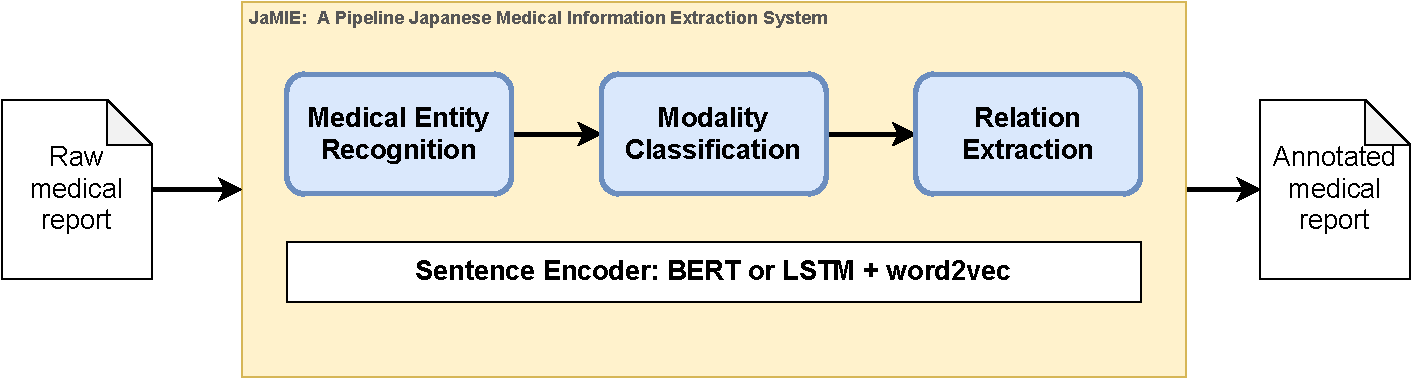
\includegraphics[width=1\textwidth]{figures/jamie.pdf}
	\caption{JaMIE működési folyamata \cite{jamie}}
\end{figure}

\subsection{Exploring the Potential of Twitter to Understand Traffic Events and Their Locations in Greater Mumbai, India \cite{twitter-traffic}}

Az információ kinyerés egy másik alkalmazása a Twitter platformon megosztott közúti balesetek valós idejű gyűjtése vagy ábrázolása. Ehhez a szerzőpáros első lépésként klasszifikálta a friss tweet-eket, majd kinyerték belőlük a névelemeket, kifejezetten a helyszínt. A klasszifikációhoz több klasszikus modellt is összehasonlítottak, melyek közül az SVM bizonyult leginkább ígéretesnek. A helyszínek kinyerésére egy kész megoldást - a StanfordNER-t - kombinálták egy saját adatukon tanított OpenNLP modellel és szabályalapú módszerekkel.

\subsection{RESIN \cite{resin}}

Egy másik terület, ahol hasonló információ kinyerő feladatról lehet beszélni: a hírek elemzése. A RESIN egy olyan rendszer, ami többféle nyelven írt szövegekből, de akár videós anyagokból képes entitásokat és történéseket kinyerni. Az entitások, valamint a köztük fennálló kapcsolatok kinyeréséhez BERT modellt használtak. Események kinyeréséhez dokumentum szinten alkalmazták a BART modellt. Az entitásokat és eseményeket a koreferencia feloldás mellett hozzákötötték a WikiData nevű tudásbázishoz. A megoldás érdekessége, hogy mindezt egy egyszerűen telepíthető Docker konténerként tették elérhetővé GitHub-on.

\begin{figure}[H]
	\centering
	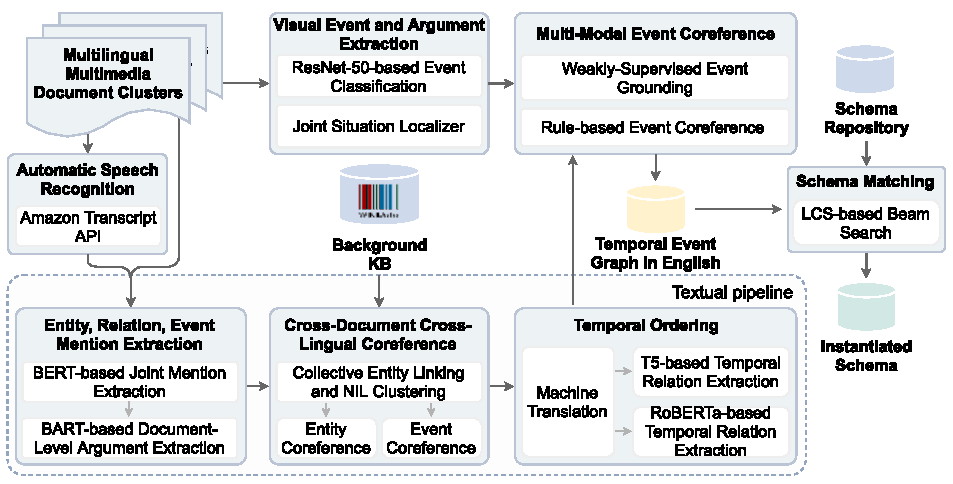
\includegraphics[width=1\textwidth]{figures/resin.pdf}
	\caption{RESIN működési folyamata \cite{resin}}
\end{figure}

% \subsection{Klasszikus módszerek}
% nem  kell
% Egyik első technika szöveg vektorrá alakítására a BoW (Bag of Words) tokenizáció volt, ami a szavak előfordulási gyakoriságát használja, viszont azok sorrendiségét teljesen figyelmen kívül hagyja. Ennek a továbbfejlesztése az N-gram modell, ami már szópárokban gondolkodik, így pontosabban képes szókapcsolatokat reprezentálni. Klasszifikációs feladatoknál még nagy javulást jelentett a TF-IDF módszer. Ez aszerint súlyozza az egyes kifejezéseket, hogy mekkora azok előfordulási aránya az aktuális dokumentumban és az összes dokumentum között.

% A neurális hálók elterjedése a szövegelemzés más területeihez hasonlóan itt is nagy áttörést jelentett. Már a konvolúciós hálók is képesek voltak jobb eredményt elérni a klasszikus módszereknél.
\chapter{Előkészületek}

\section{Adathalmazok összeállítása}

A kitűzött céljaimhoz magyar nyelven nem állt rendelkezésre publikus adathalmaz, ezért nekem kellett ilyet összeállítanom.

\subsection{Adathalmaz háttere}

Feladatom során egy K-Monitor nevű antikorrupciós civil szervezet sajtóadatbázisának bővítését segítő rendszer fejlesztését tűztem ki célul. A szervezet évek óta gyűjt a magyar sajtóból korrupcióval és átláthatósággal kapcsolatos cikkeket az adatbázisba. Az eredeti cikkre mutató hivatkozás mellett a következő metaadatok is feljegyzésre kerülnek: a cikk címe, bevezetője (lead) és a cikkben előforduló releváns személyek, intézmények, helyszínek és egyéb kulcsszavak.

A sajtóadatbázist a K-Monitor tagjai valamint önkéntesei frissítik új cikkekkel, módszertanért lásd: \ref{appendix:kmonitor-methodology}.

Az adatbázis bővítésének asszisztálása mellett azt is kitűztem célul, hogy az egyes cikkekben megfogalmazott névelemek (személyek, intézmények) közti kapcsolatokat kinyerjem. Az ötletet a K-Monitor által működtetett Háló \cite{ahalo} adta, ami egy ilyen típusú kapcsolatokat gráf formában megjelenítő weboldal.

\subsection{Adat beszerzése}

Az adathalmazhoz 2023 januárjában adatbányászattal szereztem metaadatokat. Így jutottam hozzá 36 178 db mintához.

Emellett szükségem volt magukra a cikkek szövegére is. Ehhez elsősorban egy CommonCrawl nevű archiváló rendszerre támaszkodtam. Ami ott nem volt megtalálható azt a webről gyűjtöttem (HTTP GET lekérdezés az adott URL-re) vagy Wayback Machineről szereztem be.

\subsection{Adat tisztítás}

A különféle módon letöltött HTML dokumentumokból newspaper3k \cite{newspaper3k} Python könyvtárral nyertem ki a cikkekből lényeges részeket (cím, lead, törzs, kulcsszavak). Ez az eszköz statisztikai alapú nyelvi modelleket használ arra, hogy a természetes nyelvű szövegrészeket elválassza a felhasználói felület címkéitől. A megoldás nem volt tökéletes, ezért más módszereket is kellett alkalmaznom a felesleges szövegrészek kiszűrésére.

Az egyik probléma az volt, hogy a hírek törzsébe belekeveredtek hirdetések illetve egyéb - a tartalomhoz nem kapcsolódó - szövegrészletek. Erre a megoldásom az volt, hogy bekezdésekre bontottam a cikkeket és a cikkek között ötnél többször szó szerint előforduló bekezdéseket eltávolítottam. Ezen felül töröltem a gyanúsan rövid vagy hibás kódolású újságcikkeket is. Az így képzett adathalmaz 31 641 rekordot tartalmaz.

\subsection{Dokumentum klasszifikáció}

Mivel célom volt egy bináris klasszifikáció aszerint, hogy a cikket számunkra érdekes témában írták-e, az adathalmazba kellettek nem korrupcióról vagy átláthatóságról szóló cikkek is. Azonban ehhez nem rendelkeztem adattal, ezért nekem kellett ilyen mintákat gyűjtenem.

Elsőként kiválasztottam 36 012 db cikket manuális annotálásra, ezeket előannotáltam egy korábban tanított klasszifikációs modellel. Kiválasztottam 20 000 mintát, amit előannotálás során a modell leginkább negatívnak ítélt és ezeket negatívként beemeltem a korpuszba. Ezzel az volt a célom hogy manuálisan kevesebbet kelljen annotálnom, a művelet ára az volt, hogy hamis negatívok is bekerülhettek az adathalmazba.

A tanító- és validációs halmaz számára manuálisan annotáltam (a leginkább pozitívnak ítélt) 6 000 cikket és a teszthalmazhoz külön 2 000-et (szűrés után 1 921 db negatív minta). A teszthalmaz negatív felét csak ezek a manuálisan annotált minták adták.

Végezetül a pozitív példákkal együtt egy 55 867 rekordot tartalmazó adathalmaz keletkezett.

\subsection{Névelem klasszifikáció}

Habár a korábban részletezett adathalmaz tartalmazta a releváns személyek listáját, negatív minták nem voltak benne. Ezért elsőként futtattam egy entitásfelismerést a cikkeken HuSpaCy-vel \cite{huspacy}, így hozzájutottam a cikkben szereplő összes személyhez. Innentől pedig már a két halmaz különbsége adta a negatív mintákat.

Összesen 64 000 mintát sikerült így gyűjtenem, melyből 23 000 pozitív és 41 000 negatív.

\subsection{Kulcsszó "generálás"}

A kulcsszavak megállapításához minden szükséges adathoz hozzájutottam az adatbányászattal, ezzel további feladatom nem volt.

\subsection{Reláció kinyerés}

Az egyes névelemek közti relációkkal kapcsolatban eredetileg semmilyen adattal nem rendelkeztem a nyers szövegeken kívül, ezért itt szintetikus adathalmaz összeállítása mellett döntöttem. Ez abból állt, hogy a feladatot megoldattam egy polcról levehető nagy nyelvi modellel és a megoldásokra építve egy lokális nagy nyelvi modellt tanítottam. Ezen a ponton felmerülhet a kérdés, hogy miért nem használtam egyszerűen az eredeti modellt? A válasz az, hogy sok felhasználás esetén egy lokális modell praktikusabb, mert nagyobb kontrollt kapunk a működése felett. Emellett még kevesebb erőforrást is igényel, tehát gazdaságosabb.

Elsőként felbontottam bekezdésekre az újságcikkeket és előszűrtem, csak azokat megtartva, amik tartalmaznak legalább három entitást.

\begin{figure}[H]
	\centering
	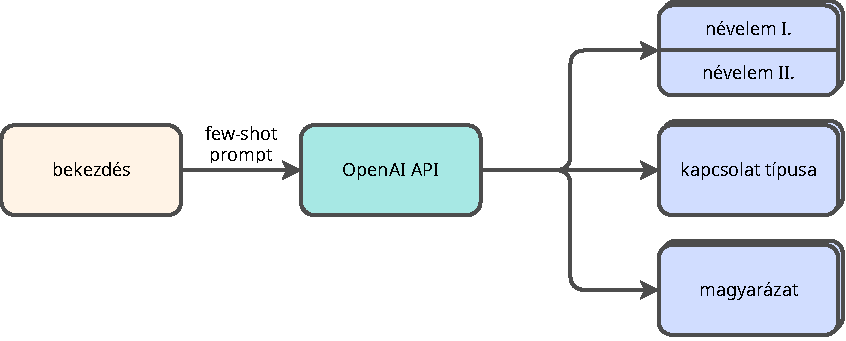
\includegraphics[width=1\textwidth]{figures/re-dataset.pdf}
	\caption{Relációkinyerési adathalmaz készítése OpenAI API segítségével}
\end{figure}

Az adathalmaz generálásához az OpenAI API-on keresztül elérhető GPT-4 turbo (gpt-4-1106-preview) és GPT-3.5 modelleket használtam. Few-shot módszert használtam a promptoláshoz. Az elvárt információ a két entitás megnevezése és a kapcsolat típusának megnevezése volt, de még egy magyarázatot is kértem a modelltől, ami egy rövid bekezdés volt.

\begin{figure}[H]
	\centering
\begin{tabular}{rrrr}
	& train & validation & test \\ \hline
	GPT-3.5 & 500 & 50 & 50 \\
	GPT-4-turbo & 600 & 60 & 60 \\
\end{tabular}
\caption{relációkinyerési adathalmaz eloszlása}
\end{figure}

\section{Kísérletek elemzése}

\subsection{Tanítási környezet}

Minden finomhangolási kísérletet egy Nvidia RTX 3060 (12GB) videokártyán végeztem. A kísérletezés átláthatóbbá tételéhez axolotl szoftvert használtam, ami lehetővé teszi, hogy egy konfigurációs fájl kitöltésével finomhangoljunk modelleket.

\subsection{Klasszifikációs módszerek összehasonlítása}

Klasszifikációs feladatra két mély-tanuláson alapuló módszert vizsgáltam meg: BERT és GPT modellek finomhangolását. A két megoldás lényegében abban különbözik, hogy míg a BERT kifejezetten támogat klasszifikációs feladatokat, addig a GPT kizárólag szöveggenerálásra képes. Viszont a klasszifikáció visszavezethető szöveggenerálási problémára, így kihasználhatjuk a GPT modellek nagyobb paraméterszámát pontosabb eredmények elérésére.

Ami viszont egy hátránya a GPT modelleknek, hogy a nagyobb paraméterszám miatt több számítási kapacitással jár a használatuk.

\begin{figure}[H]
	\centering
	\begin{tabular}{rrrr}
		modell & precision & recall  & accuracy \\ \hline
		PULI-GPT-3SX & 0.776 & 0.878 & 0.966  \\
		llama 7B & 0.860 & 0.810 & \textbf{0.971} 	\\
		huBERT & 0.739 & 0.950 & 0.963 \\
	\end{tabular}
	\caption{klasszifikációs modellek kiértékelése}
\end{figure}

\begin{figure}[H]
	\centering
	\begin{tabular}{rrrr}
		modell & gpu* inference & cpu** inference \\ \hline
		PULI-GPT-3SX & 1.90 it/s & 0.03878 it/s \\
		huBERT & 126.85 it/s & 7.10 it/s \\
	\end{tabular}
	\caption{klasszifikációs modellek teljesítménye}{
		* Nvidia 3060 12gb
		** Ampere A1 (Oracle cloud)}
\end{figure}

\subsection{Névelem klasszifikáció kiértékelése}

Névelem klasszifikációra az adathalmaz sajátosságai miatt túlságosan komplex feladat lett volna BERT modellt tanítani, ezért itt kizárólag GPT-t használtam. Ezt úgy vezettem vissza szöveggenerálási feladatra, hogy a prompt elején átadtam a HuSpaCy által felismert entitások listáját és utána a cikk szövegét.

\begin{figure}[H]
	\centering
	\begin{tabular}{rr}
		modell & accuracy \\ \hline
		személyek & 0.8523 \\
		intézmények & 0.8384 \\
	\end{tabular}
	\caption{Névelem klasszifikációs modellek pontossága}
\end{figure}


\subsection{Reláció kinyerés}

Relációkinyeréshez az OpenAI modellek működésének reprodukálását tűztem ki célul, ezért itt adta magát egy GPT modell finomhangolása. Az viszont már nem volt teljesen egyértelmű, hogy melyik alap modell a legalkalmasabb. Kifejezetten magyar nyelvre tanított GPT modellek közül a PULI-GPT-3SX jöhet szóba, de számos többnyelvű modell jelent meg azóta fejlettebb architektúrával. Sajnos szerzői jogi okokból a modellek megosztói ellenérdekeltek a pontos tanítási adat megosztásában. Így gyakran nem tudni mennyi magyar nyelvű adatot látott egy GPT. Egy ilyen többnyelvű modell a Mistral 7B, ami a llama architektúrára épül és azt még számos új módszer beépítésével tökéletesíti. Azért, hogy össze tudjam hasonlítani a Mistral 7B-t és a modelleket, kiértékeltem mindkettőt két magyar nyelvű benchmarkon.

\begin{figure}[H]
	\centering
	\begin{tabular}{rrrr}
		modell & hucola F1 & husst F1 \\ \hline
		PULI-GPTrio & 0.523 & 0.541 \\
		PULI-GPT-3SX & 0.366 & 0.625 \\
		Mistral-7B & \textbf{0.872} & \textbf{0.636} \\
%		RWKV-World-3B & 0.865 & \textbf{0.675} \\
	\end{tabular}
	\caption{GPT modellek magyar benchmarkokon few-shot (N=5)}
\end{figure}

A kiértékelés kapcsán meg kell jegyeznem, hogy a validációs (dev) halmazt használtam, mivel a teszt minták megoldása nem nyilvános.

Mivel ennél a feladatnál nem lehet az eredeti adathalmaz megoldásában megbízni, a modell kimenetét manuálisan értékeltem ki. TODO

\subsection{Kulcsszó kinyerés eredmények}

Ebben a kulcsszókinyerési feladatban nagyon sok lehetséges kulcsszó közül kell kiválasztani az adott szövegre illőket. A sok lehetséges osztály miatt itt a BERT modellt nem találtam megfelelőnek, ezért csak GPT modellt tanítottam.

Ugyanehhez a problémához a K-Monitor által egy SpreadMonitor nevű cég számára szervezett hackathon alatt is készült egy megoldás klasszikus módszerekkel. Ez a megvalósítás BoW tokenizációra épül és Random Forest-et használ klasszifikációra. Erőssége, hogy jobb eredményeket ér el, mint a GPT-t alkalmazó megoldás, viszont cserébe minden osztályhoz külön bináris klasszifikációt kell végeznie.

\begin{figure}[H]
	\centering
	\begin{tabular}{rrrr}
		kulcsszó & GPT & BoW + RandomForest \\ \hline
		önkormányzat & 0.60 & \textbf{0.66} \\
		klientúra & 0.55 & \textbf{0.68} \\
		közbeszerzés & 0.69 & \textbf{0.74} \\
		ingatlan & 0.71 & 0.71 \\
	\end{tabular}
	\caption{F1-score eredmények néhány kulcsszóhoz}
\end{figure}

\chapter{Rendszer megvalósítása}

\begin{figure}[H]
	\centering
	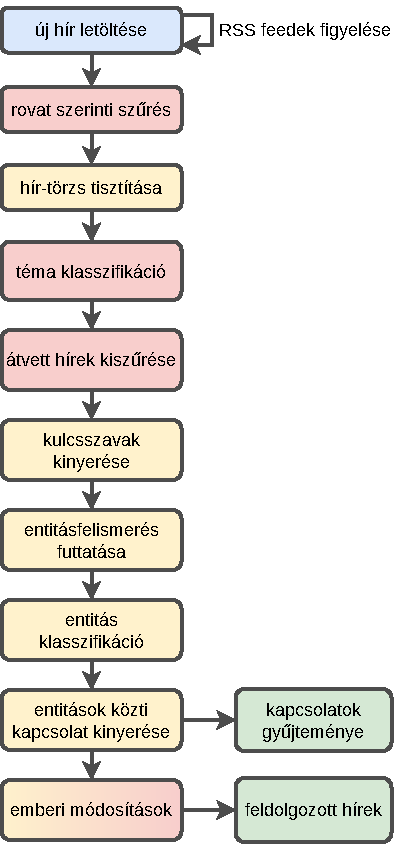
\includegraphics[width=80mm,keepaspectratio]{figures/flowchart-konkret.pdf}
	\caption{Rendszer működését bemutató folyamatábra}
\end{figure}

\section{Rendszer összeállítása}

\subsection{Modellek felkészítése telepítésre}

\subsection{Modulok összekapcsolása}

\subsection{Webes felület}

\chapter{Összegzés}

\section{Rendszer működése}

A tervezett rendszer különálló modulokból épül fel, amik lehetnek kész általános modellek finomhangolt nagy nyelvi modellek vagy csak egyszerű szabály alapú megoldások...

\section{Értékelés}

\section{További lehetőségek}

% felhsznaloi szemmel?
%----------------------------------------------------------------------------
\chapter*{Köszönetnyilvánítás}\addcontentsline{toc}{chapter}{Köszönetnyilvánítás}
%----------------------------------------------------------------------------

Szeretném megköszönni a konzulensemnek, \vikkonzulens nak a segítséget, amit három félév óta nyújt.

%\listoffigures\addcontentsline{toc}{chapter}{Ábrák jegyzéke}
%\listoftables\addcontentsline{toc}{chapter}{Táblázatok jegyzéke}

\bibliography{mybib}
\addcontentsline{toc}{chapter}{Irodalomjegyzék}
\bibliographystyle{plain}

\appendix

\chapter*{Függelék}\addcontentsline{toc}{chapter}{Függelék}
\setcounter{chapter}{6}  % a fofejezet-szamlalo az angol ABC 6. betuje (F) lesz
\setcounter{equation}{0} % a fofejezet-szamlalo az angol ABC 6. betuje (F) lesz
\numberwithin{equation}{section}
\numberwithin{figure}{section}
\numberwithin{lstlisting}{section}
%\numberwithin{tabular}{section}

\section{K-Monitor módszertana}
\label{appendix:kmonitor-methodology}

\emph{A következő egy minimálisan módosított kivonat a módszertanukból}:


Új cikk felvételének az alábbi kritériumai vannak:

\begin{enumerate}
	\item konkrét korrupciós esetet ír le
	\item cikk szerzője állítja/sugallja, hogy valaki a ráruházott hatalmat saját maga, vagy egy harmadik fél hasznára fordította
	\item cikk korrupciós ügyben történő jogi eljárásról tájékoztat
	\item korrupciós vádat cáfolnak vagy védekeznek
	\item következő témák esetében szabálytalanságok merülnek fel: közbeszerzés, pártfinanszírozás, pályázatok, kormányzat szerv vagy állami vállalat gazdálkodása, vagyonosodás, juttatások, privatizáció, whistleblowing
	\item következő kifejezések közül valamelyik előfordul a cikkben: korrupció, sikkasztás (közszolga által), hűtlen kezelés, vesztegetés, hivatali visszaélés, hatalommal való visszaélés, befolyással üzérkedés, hanyagság, adócsalás, számviteli fegyelem megsértése, protekció, nepotizmus, jogosulatlan gazdasági előny, versenykorlátozás, kartell, whistleblowing/közérdekű bejelentés, közérdekű adatok, átláthatóság
\end{enumerate}

Felvételt kizáró okok:
\begin{itemize}
	\item pártközlemény
	\item publicisztika
	\item mocskolódás
	\item nem saját anyag, más lapra hivatkozik és nem tartalmaz új információt
\end{itemize}

A cikkeket metaadatokkal is ellátták az alábbiak szerint:

\begin{itemize}
	\item Személyek: aki a cikk alapján negatív összefüggésbe hozható az eseménnyel, vagy korábban negatív összefüggésbe hozták, és tisztázták a vádak alól.
	\item Intézmények: a cikk szerint a cselekményben érintett cég, hivatal, szervezet (gazdaság, politika, társadalom) - tehát itt is csak a negatívan említettek!
	\item Helyek: ha mérvadó az ügy helyszíne (település/megye/ország). Csak akkor alkalmazzuk, ha az ügy szempontjából releváns és állami/önkormányzati szereplőről van szó.
	\item Egyéb kulcsszavak: az ügy témakörét adja meg, fontos jellemzőket rögzít. 
\end{itemize}

\clearpage\section{Használt promptok}

\subsection{Címkék generálása}

\begin{verbatim}
[címkék generálása]
{title}

{description}

{text}

cimkék: {keywords}

###

korrupciós címkék: {output}
\end{verbatim}

\subsection{Entitás klasszifikáció (személyek)}

\begin{verbatim}
[személy klasszifikáció]
{text}

###

összes: {all}
korrupcióban érintett: {output}
\end{verbatim}

\subsection{Entitás klasszifikáció (intézmények)}

\begin{verbatim}
[intézmény klasszifikáció]
{text}

###

összes: {all}
korrupcióban érintett: {output}
\end{verbatim}

\subsection{Reláció kinyerés}

\begin{verbatim}
Bekezdés:
"{text}"

Relációk:
{output}
\end{verbatim}

ahol az output az alábbi struktúrájú objektumokat tartalmazó tömb:

\begin{verbatim}
Indoklás: {explanation}
Kapcsolat: {relation}
Tárgy: {subject}
Alany: {object}
\end{verbatim}

\label{page:last}
\end{document}
